\chapter{Background and Related Work}
Since the Delay-Tolerant Network architecture is first introduced, its security concerns have drawn the attention of relative research groups. Soon, much effort has been put on analysing the practicality of security implementation in DTNs and many designs have been made. Here two of security protocols which considered similar to this project are introduced as references.

\section{Delay-Tolerant Networks (DTN)}
Comparing to Internet which is relatively stable and reliable, so called ``challenged networks" are characterized by latency, bandwidth limitations, error probability, node longevity, or path stability that are substantially worse than is typical of today’s Internet \cite{Kevin}. The reason for causing the networks ``challenged" could be various - from geographical distances, lacking infrastructure to extreme environment conditions. Examples of such networks have been given by Fall, such as exotic media network - like near-earth satellite communication, and military ad-hoc networks. In order to achieve successful communication within such networks, instead of using TCP/IP - which will behave disappointingly \cite{Scott}, each challenged network may introduce its own protocol suits and network architectures to meet their specific needs. However, the diversity of these various protocols and architectures prevents those networks to communicate with each other and it has been justified by Fall \cite{Kevin} that simple link-repair approaches is not sufficient to solve the whole problem.

Then the architecture of Delay-Tolerant Network (DTN) was introduced to tackle the problem. Basically it achieve communication between various disparate challenged networks with significantly different sets of physical and operational constraints (latency, stability, etc.) by adding another layer of protocol to the local protocol stack. The Figure \ref{fig:dtn} briefly illustrates the architecture of a delay-tolerant network.

\begin{figure}[h!]
\centering
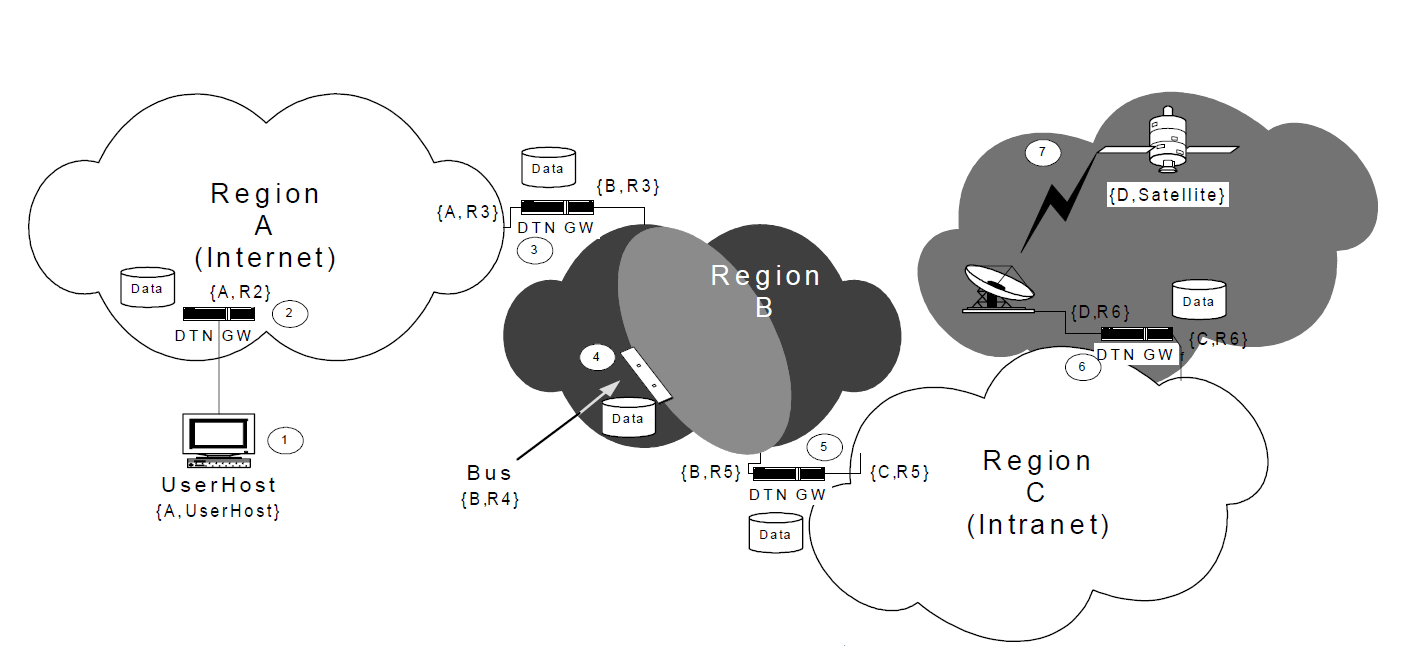
\includegraphics[width=\textwidth,natwidth=1420,natheight=672]{figures/dtn.png}
\caption{Overview of a Delay-Tolerant Network, cited from \cite{Kevin}}
\label{fig:dtn}
\end{figure}

It separates different challenged networks into ``regions" - within each region, nodes communicate under a same protocol, while different regions may run different protocols. As shown in the figure, region A uses Internet, region B uses a bus to deliver messages, region C uses its own Intranet and region C uses satellite to communicate. Different regions are connection by DTN gateways where messages from one region will be routed and forwarded to another region.

One of the key concept of DTN is custody transferring, which refers to the delivery of message from one DTN hop to another together with its reliable delivery responsibility - it's very much like delivering packages through a postal service. And using message couriers to achieve such custody transfer has been accepted as one practical implementation to overcome the difficulties in DTN \cite{Jain}\cite{Zhao}. Although the security issues of DTN have been discussed and evaluated in the high level design of the architecture \cite{Cerf}\cite{Scottrfc} (mainly to maintain efficient routing and prevent abuse of DTN), many security concerns still remain to be considered in the specific courier-dependent message delivery scenario (like what if the courier could be hijacked and examined?). Referencing the high level security framework pre-defined in the architecture, this project will dive into the detail of courier-dependent message delivery and create a practical and efficient security protocol for such scenario.

\section{Deniable Authentication}
Privacy protection has been taken much attention to since the communication through digital networks grows dramatically. Most network protocols require authentication as one of its essential steps to achieve secure communication. However, common authentications do not take privacy as one of its goals, thus they require revealing unique identifier of an entity to prove its identity to others - such like a digital signature or a piece of plaintext whose ciphertext can only be decrypted by the entity. As a matter of fact, it is this authentication mechanism disclose the identity of authenticator to third parties. Conversely, in many cases entities want to authenticate themselves to the target entities without revealing their identities to any third parties. This issues have been investigated and analysed by Abadi, who consequently introduced ``private authentication" and presented protocols meet the requirements \cite{Abadi}.

The concept of deniable authentication is created even earlier, by Dwork and Sahai \cite{Dwork}. It indicates the situation that an entity wishes to authenticate a message to the target entity while no any other entities can verify the authentication. Namely, the target entity can not prove the authenticity of the origin of the message to any other entities even itself is convinced by the authentication, thus the message creator can fully deny the existence of the message. It is extremely powerful in terms of privacy protection as combining with privacy authentication, no any private information will be leaked during the authentication. And its repudiation property is proved useful in applications like voting systems and commercial negotiation systems.

So far, many deniable authentication protocols have been invented, they can be sorted as two main classes - interactive \cite{Borisov} and non-interactive \cite{Xin}\cite{Wang}\cite{Shao}. Interactive deniable authentication requires at least 2 messages exchanged during the protocol, one forward and one reply. While non-interactive deniable authentication can achieve the goal in just one message with the cost of heavier computation.

This feature is added in the CDSP to provide an extra level of security to the message being exchanged in order to against potential malicious operations of couriers and message recipients. It might be very important in circumstances like military network or secret message delivery missions.

\section{Bundle Security Protocol \cite{Symington}}
Soon after the release of DTN architecture specification \cite{Cerf}, a protocol called Bundle Protocol \cite{Scottrfc} is designed and documented by Scott et al., which formally defines the format of messages (named bundles) exchanged between each end-to-end entities and abstracts the services provided by DTNs. Analogous to TCP/IP providing end-to-end connectivity specifying how data should be formatted, addressed, transmitted, routed and received between originator and destination in Internet, Bundle Protocol takes care of those issues for every DTN hops. Figure~\ref{fig:bundleblockformat} shows the the basic block formats in bundle protocol. Basically, it defines that a single bundle should contain one primary bundle block and arbitrary number of bundle payload blocks. The primary bundle block is highly formatted, it describes the information about the whole bundle,  while each bundle payload block provides different services that can be totally independent to each other and its format is relatively free to extend. This message structure is designed for extension as new functions could be easily added to the protocol by defining another now type of bundle payload block.

\begin{figure}[h!]
\centering
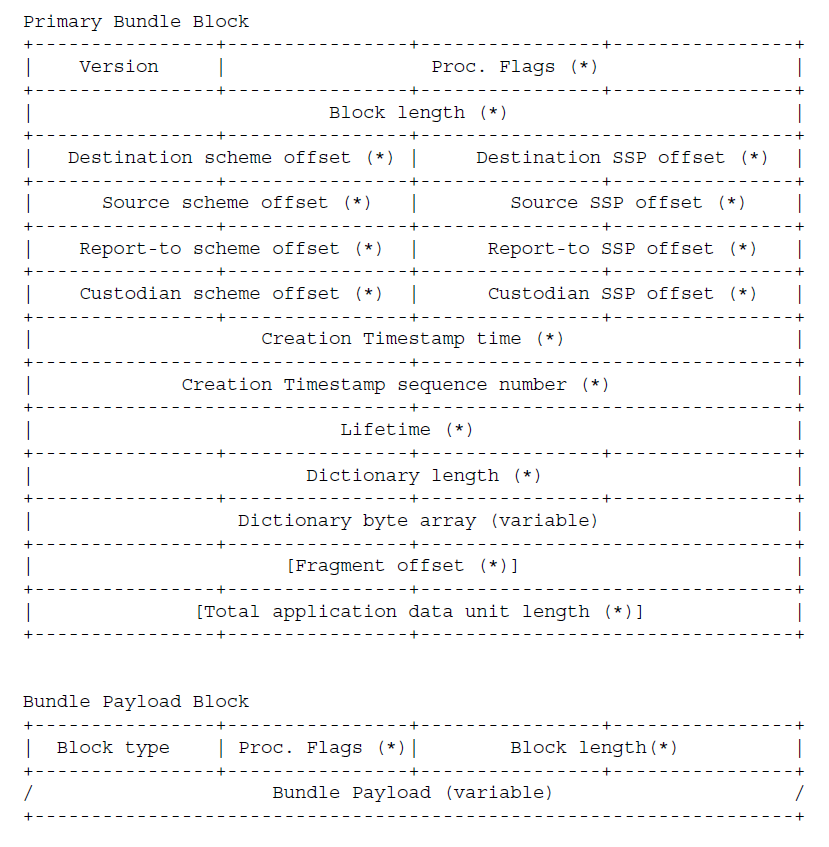
\includegraphics[width=\textwidth,natwidth=829,natheight=847]{figures/bundleblockformat.png}
\caption{Message Format of Bundle Protocol \cite{Scottrfc}}
\label{fig:bundleblockformat}
\end{figure}

The Bundle Security Protocol is one of extensions of Bundle Protocol. It is designated to provide data integrity and confidentiality protection for the Bundle Protocol. The main contribution is defining 4 new types of bundle payload block - BundleAuthenticationBlock, PayloadIntegrityBlock, PayloadConfidentialityBlock and ExtensionSecurityBlock. Those new types of blocks - as their name stated, can be appended to any bundle to add an extra level of corresponding security protection to it. For example, if a bundle needs to be authenticated, the originator should add an extra bundle payload block to the original bundle, formatted as a BundleAuthenticationBlock. Thus the authentication of the bundle can be checked in every DTN hop during the transmission.

We can see that Bundle Security Protocol has defined the security issues in a high level, it ensures the secure message transmission between originator and receiver connected by hops. However, the detailed operations between hop to hop is not covered by this protocol. Referring to the architecture of DTN, every end-to-end nodes are linked by hops, and the message transmission from one hop to the next is called custody transfer. The implementation of custody transfer can be various, but a common method is courier-dependent transferring. In Bundle Security Protocol, such custody transferring is assumed to be accomplished securely and efficiently so that it only cares the higher level issues. Unfortunately, it is not always the case. Every custody transferring can be complicated and extra work should be done to keep it functioning. Thus this project will explore the specific scenario of courier-dependent custody transferring and create a protocol for it. Although the message format of Bundle Security Protocol is highly referential, it still not quite fit the scenario. The major problem is: as a general protocol it has a very heavy overhead to maintain the consistency of different blocks and extensions, which seems redundant in the specific courier-dependent scenario. So comparing to the Bundle Security Protocol, the newly created protocol will use less-sized messages and be more problem specific.

\section{DTN Anonymity and Secure Architecture \cite{Kate}}
The DTN Anonymity and Secure Architecture (DASA) is inspired by Seth et al. who tried to find a secure solution for helping rural areas to get continuous Internet access despite the long-period disconnection \cite{Seth}\cite{SethKeshav}. Although many different situations may arise in rural areas, Seth et al.'s study focuses on a particular example of them: buses with wifi-based access and storage capability periodically drive past each villages and collect data from users in villages. Then buses carry the data to the nearest local Internet gateway and send out the data collected. Figure~\ref{fig:ruralarea} roughly illustrates the scenario. Basically, Seth et al.'s architecture achieves the secure communication between each user and buses in such a way that every data delivery from user to bus must be mutually authenticated. Based on this achievement, Kate et al. abstracts the scenario such that it not only applies to rural area networks but also any generic DTNs. Furthermore, Kate et al. also adds two more security properties to the original architecture - data confidentiality and anonymity, forming the DTN Anonymity and Secure Architecture.

\begin{figure}[h!]
\centering
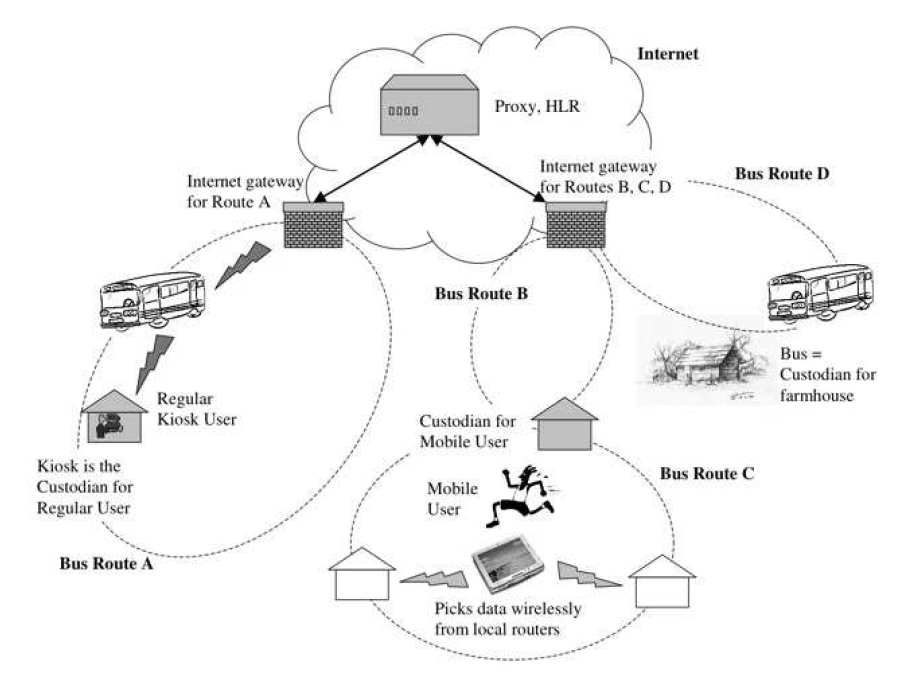
\includegraphics[width=\textwidth,natwidth=913,natheight=682]{figures/ruralarea.png}
\caption{Rural Area DTN \cite{Seth}}
\label{fig:ruralarea}
\end{figure}

The DTN Anonymity and Secure Architecture is very close to the scenario of this project, as it takes care of the authentication processes between end users and couriers - here the buses, and conceals the identity of end users. However, there are still some points remain controversial: (1) It does not hide the message content from the DTN router (courier), so the message content will be totally exposed once the DTN router is compromised. (2) It requires mutual authentication when end node transmit message to a DTN router (courier). Normally, mutual authentication is interactive or it demands for extra assumptions - such as Sakai-Ohgishi-Kasahara (SOK) Key Agreement Scheme \cite{Sakai}, which leads to computational complexity, thus one way authentication might be a better choice. (3) Its anonymity mechanism highly relies on a trusted third party ``private key generator" which may or may not be introduced in the system. (4) The message sent from end users is not fully deniable. According to the specification of its anonymity mechanism, it only conceals the sender identity behind a group of valid users identities. Although the courier does not know the true identity of sender, it at least can prove that one of the member in the group created the message to a third party.